% -*- root: ../thesis.tex -*-

\chapter[Introduction]{Introduction}
\label{ch:intro}

\section{From actor \emph{modelling} to actor \emph{programming}}
\label{sec:intro:abs}

Object-oriented programming~\cite{booch1982object,meyer1988object} has been of one the dominant paradigms for software engineering in the past three decades.
One object interacts with another object using the notion of a method.
Method invocations are \emph{blocking}; i.e. the caller object waits until it receives the result of the method call from the callee object.
Surprisingly, this model of interaction was \emph{never} the intention of the creator of the paradigm.
Originally, object interactions were meant to be \emph{messages} among objects and objects behaved as autonomous entities possibly on remote locations on a network; Alan Kay clarified later~\cite{alank1,alank2}. 
On the contrary, almost all the object-oriented languages at hand have followed the blocking and synchronous model of messaging based on a common misunderstanding. 
The original definition of object-oriented programming is close to another model of computation: actor model.  

One of the fundamental elements of actor model~\cite{actors:agha,agha97} is \emph{asynchronous} message passing.
In this approach, interactions between objects are modelled as \emph{non-blocking} messages.
One object, the sender, communicates a message to the other object, the receiver.
At the receiver side, a message eventually leads to a method invocation (in the object-oriented paradigm) or a function call (in the functional paradigm).
In the actor model, the locality of the objects is not visible in the messages.
A system is composed of objects with communicating messages.

A considerable amount of research has been carried out to mix object-oriented programming languages with the actor model. 
Language extensions, libraries, and even new programming languages are the natural outcomes of such research.
The more mainstream the language, the more research and development are available in the intersection of object orientation and actor model.
For example, \cite{actor_frameworks_jvm:agha} presents a comparative analysis of such research for Java and JVM languages.

The rapid increase of computational power added a new aspect added to create a triangle: object-oriented, actor model, and \emph{concurrency}.
Concurrency makes it harder to verify programs in terms of correctness of runtime behavior. 
Scheduling of object messages in threads of executions is one of main challenges.
In addition, in the presence of scheduling and thread interleaving, it is important that objects are able to protect their state from concurrent modifications for correctness properties.
In this thesis, we take advantage of a modelling language that aims to mix the three aspects in addition to the capabilities of formal semantics and verification.

ABS~\cite{johnsen2012abs,hahnlehjlssw11} is a modelling language for concurrent objects and distributed systems.
ABS is based on the semantics of the actor model~\cite{actors:agha}.
ABS language provides a set of core features including algebraic data types (ADT), a functional layer, and a concurrency layer.
The ABS concurrency layer uses co-operative scheduling of active objects~\cite{creol:broch:owe}.
ABS semantics is completely expressed in structural operational semantics~\cite{plotkin:sos}.
This allows ABS models to take advantage of various verification methods and static analysis techniques.
% 
Co-operative scheduling in ABS has been additionally extended for real-time scheduling taking priorities and time constraintsinto account~\cite{bjork2013:rtabs,johnsen2012modeling}.
Thus, in general, ABS concurrency layer is a perfect fit if it can be integrated with industry-level real-world programming languages.
% With distributed computing as one of the recent de-facto requirements in every business use case, an enormous effort has gone to improve the current mainstream programming languages to fit for the new requirements of distributed and concurrent sett1ings.

Considering the mainstream programming languages
\footnote{\url{http://www.tiobe.com/index.php/content/paperinfo/tpci/index.html}}, Java~\cite{gosling2000java} is one of the most commonly-used.
Since Java 1.5 and the rise of the concurrency API in Java~\cite{jsr166}, substantial effort is spend by the community on how concurrency and distribution can be improved in Java, along the lines of the actor model, as provided by ABS.
However, not all the development on Java libraries and frameworks are based on a rigorous formal semantics. 
Therefore, this gives rise to issues and challenges in terms of correctness, semantic preservation, and reasoning.

% We deliver ABS concurrency layer in form of a Java library API.
% However, 
The Java language specification (JLS)~\cite{gosling2000java} clearly concludes that Java language is not comptabile and ready to be extended with a functional language that supports algebraic data types.
This has been the focus of research and development to extend Java to a functional language~\cite{odersky1997pizza,henkel2003discovering,nystrom2003polyglot,bracha1998making}.
The Scala language~\cite{odersky2004scala} is a result of the research. It is a dynamic, functional, and object-oriented language on JVM.
Although such extensions over Java towards a functional language exist, they lack formal semantics in the context of concurrency and actor model.

We primarily focus on ABS concurrency layer and deliver its semantics as a Java API.
We argue that the advantage of a correct semantic translation from ABS concurrency layer to its Java equivalent constructs overcomes the additional support of functional layer with \emph{partial} formal semantics.
Our approach enables programmers to model their Java systems in terms of ABS concurrency semantics and then create a correct mapping and implementation from ABS to Java using an API.
In addition, we aim to facilitate ways to actually program ABS models taking advantage of the standard Java libraries.

\section{Architecture}
\label{sec:intro:arch:crit}

In this section, we present a high-level overview of design goals that we pursue in this research. 
%Equivalently, the effectiveness and success of this research is measured upon the achievement of the discussed goals and objectives. 

\paragraph{Polyglot Programming}
With the rise of distributed computing challenges, software engineering practice has turned to methods that combine multiple programming languages and models to complete a task. 
In this approach, different languages with different focus and abstractions contribute to the same problem statement in different layers. 
Polyglot programming essentially enables software practice to apply the \emph{right} language in the appropriate layer of the problem statement. 
In this research, we aim to deliver ABS semantics and features in a polyglot approach. 
The programmer develops models with ABS that \emph{partially} take advantage of the target language features (e.g. from Java).
This approach is also referred to as \emph{Foreign Function Interface} in the context of ABS modelling.
Listing~\ref{lst:abs:java} shows ABS code that uses \jtt{java.util.ArrayList} as a data strucuture.
With Polyglot programming in ABS, the programmer does \emph{not} need to define the abstractions necessary for the list construct. 

\begin{lstlisting}[float=h,language=Java,caption=Using Java in ABS,label=lst:abs:java]
List<String> params = new ArrayList<>();
myObj ! doSomething(params);   
\end{lstlisting}

\paragraph{Scalability} 
Asynchronous message passing in ABS is a fit for distributed systems.
In such systems, the number of messsages delivered among actors in the 
environment is not predictable at runtime.
Therefore, distribution challenges performance efficiency or scalability.
The goal is to ensure the actor system scales in performance with least 
influence from the number of asynchronous messages delivered in the system.

\paragraph{Modularity} 
The scope of the research spans to a number of layers revolving around ABS
 language:
\begin{itemize}
\item \emph{Compiling ABS to a target programming language}
One first objective is to compile an ABS model to a target programming language.
The compilation can be at \emph{source-to-source} or \emph{source-to-bytecode}
level.
Target languages potentially include mainstream programming languages such as
Java, Erlang, Haskell, and Scala.
Thus, the ABS programmer should be able to use an ABS compiler to compile
their ABS models to the target languages.
\item \emph{Using ABS semantics as an API in a programming language}
The ABS language is precisely expressed with structural operational semantics~\cite{johnsen2012abs} in addition to its syntax definition.
The semantics of ABS can be delivered in a programming language
as Application Programming Interface (API) as long as the programming language provides sufficient constructs to respect ABS language semantics.
In addition, such ABS programming API should be \emph{verifiable}.
If an ABS mapping to a programming API is provided, a programmer is able to
take advantage of ABS semantics without directly programming in ABS.
Such capability from ABS enables industry users of mainstream languages to
model their systems in ABS semantics using their programming languages and
platforms.
\item \emph{Modelling in ABS}
ABS language provides a rigorous semantics to model concurrent
and distributed systems.
For practical purposes, the user (that can be a programmer, an analysist,
or a researcher) desires a tool-set and IDE that allows working with ABS 
models in a user-friendly way.
The ABS IDE and tool-set developers should be able to easily reuse and compose
over existing modules and components.
\end{itemize}

% Based on the scopes and layers of usage of this research, we aim to provide 
% a highly modular architecture in design and implementation.
% The goal is verifiable based on produced artifacts of this research in terms
% of their \emph{usability}, \emph{re-usability}, and \emph{composability} in
% different contexts.

\paragraph{Extensibility}
It is a common practice in software engineering that components are developed with a mixture of \emph{configuration}, \emph{extension} and \emph{composition}.
Hence, delivering the ABS language features as an API brings about a new requirement: to configure or extend the API. 
In particular, the ABS programmer should be able to extend the API to customized requirements. 
%The extensibility is provided either through configuration of the API or API extension.

\Behrooz{It's worth to include the figure but needs more work to justify its presence and how it relates to this thesis.}
Figure~\ref{fig:arch} presents the general architecture of the implementation.

\begin{figure}[h]
\centering
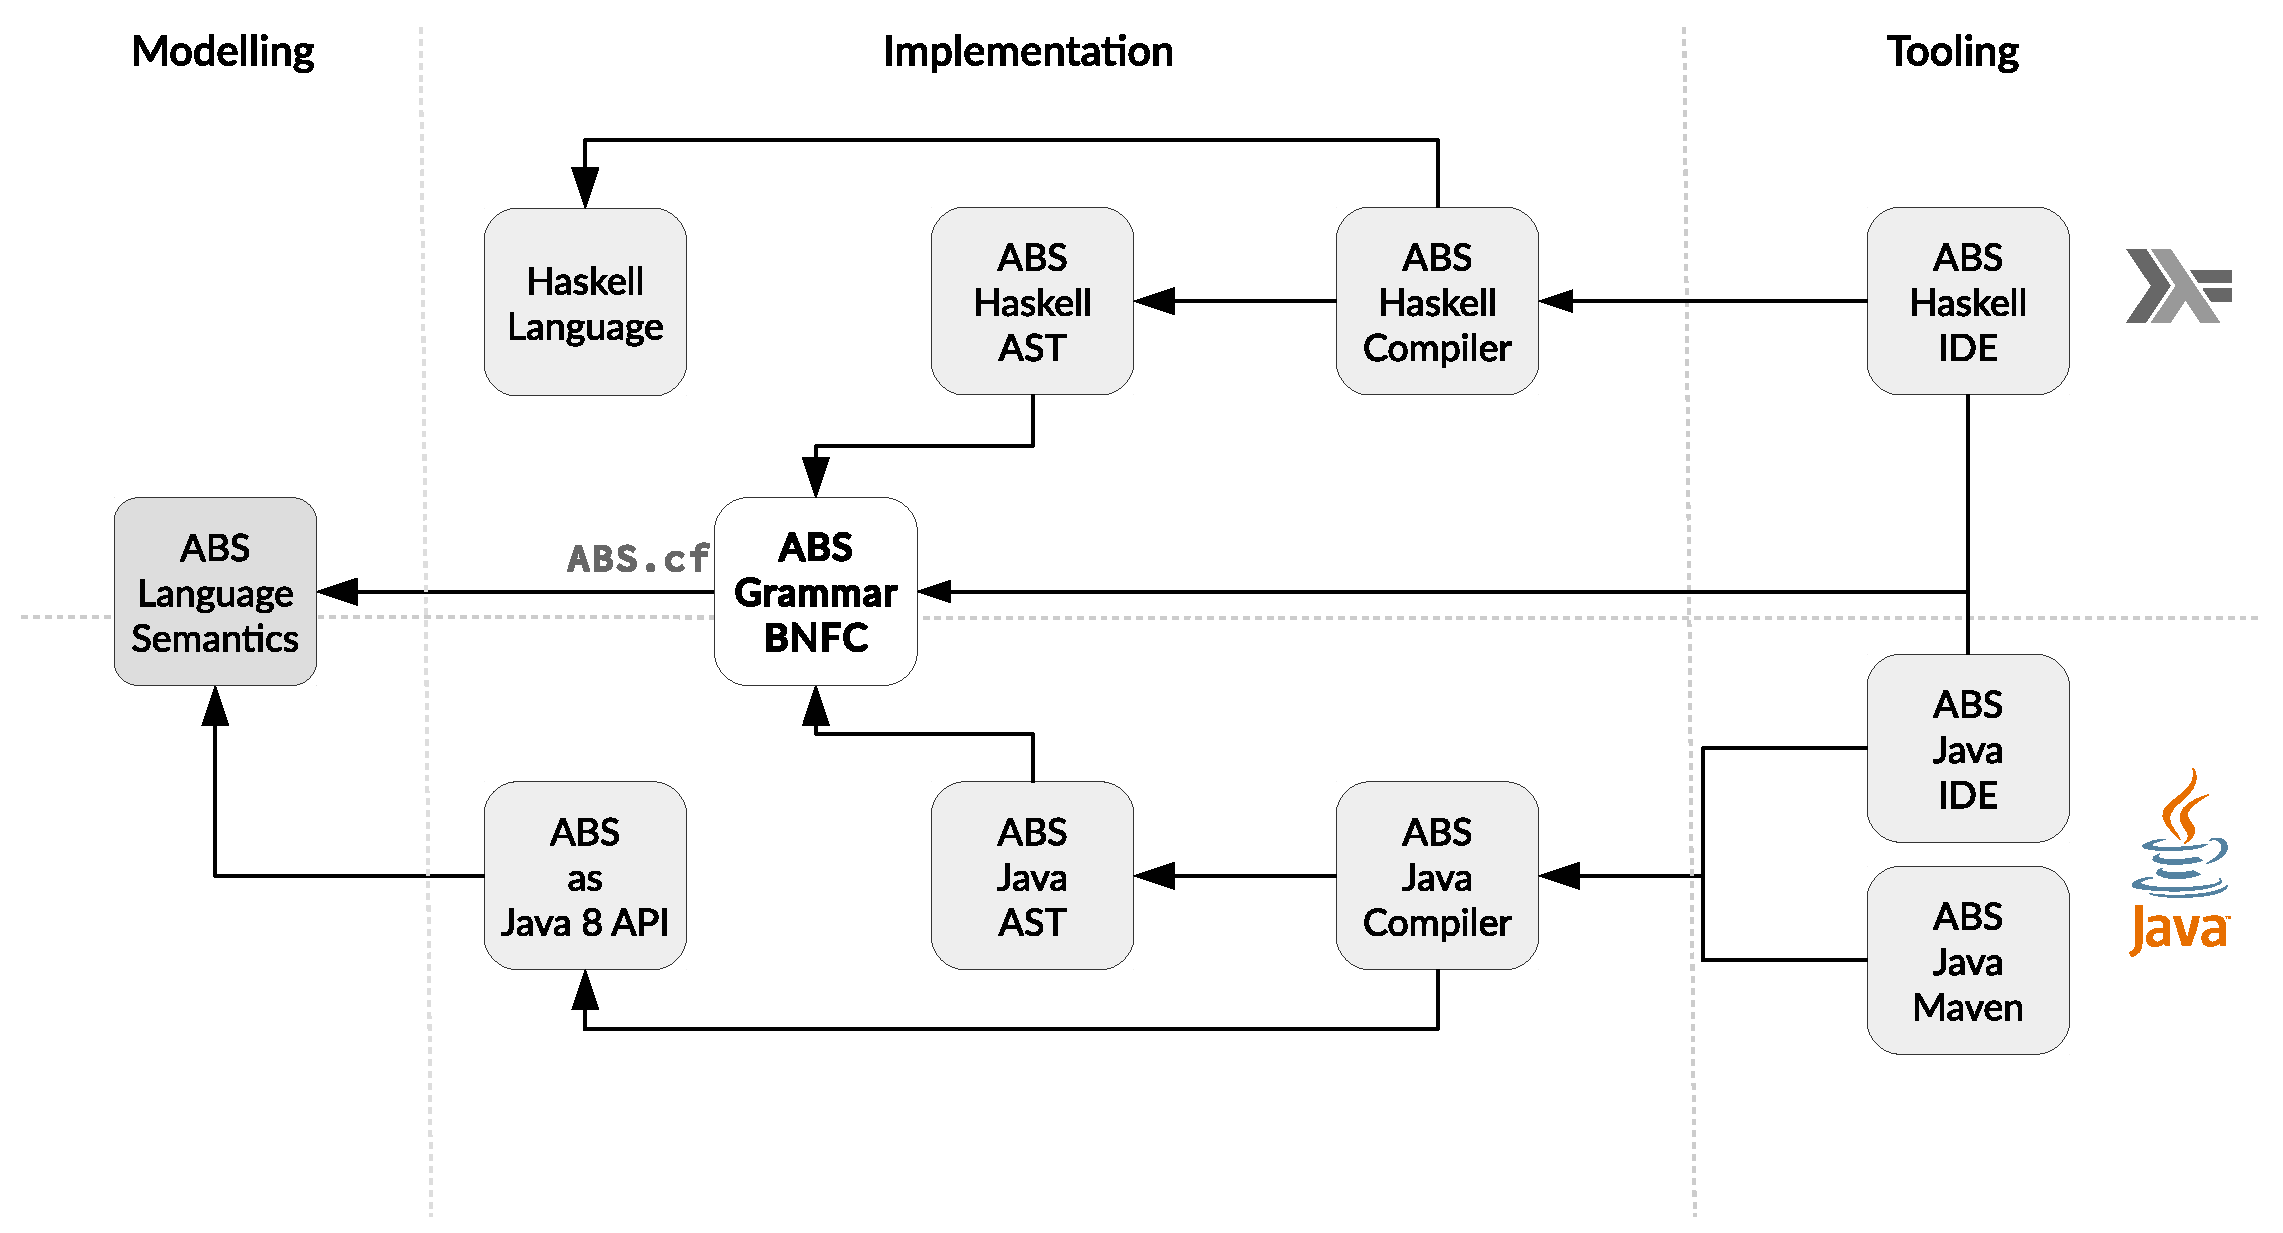
\includegraphics[scale=0.3]{../figs/Arch.eps}
\caption[General Architecture]{General Architecture of ABS API and Java Language Backend}
\label{fig:arch}
\end{figure}

\section{Literature Overview}
\label{sec:intro:rel}

We discuss a brief overview of related work in the context of programming languages, actor model, and concurrency.
We divide the overview in two levels; one is at the level of the programming languages and the other is for the external (third-party) libraries developed for programming languages.

\subsection{Programming Languages}
\label{sec:intro:proglangs}

In this section, we briefly provide an overview of the programming languages that have targetted similar problem statements.
It is important to note the timeline and the rapid evolution of programming languages trying to provide an actor-based model of asynchronous message passing.
In addition, we identify different types of research and work related to actor model and concurrency programming:
\begin{description}
\item[First-Class Citizen]
%is the type of programming languages that deliver actor model programming support as a first-class citizen of the language.
Languages in which the actor model is by-design part of the syntax and semantics of the language.
\item[Implicit By Design]
refers to the type that there is no explicit notion of actor models in the language syntax or semantics.
However, the programming language provides fundamental constructs for concurrency and asynchronous message passing.
Thus, it becomes an easy task in this kind of programming language to create an abstraction to support the actor model by coding.
\item[External Library]
refers to the type of programming languages for which actor model support is provided by an external library developed for the language.
\end{description}


Table~\ref{tbl:actor:pl} presents a summary.

\begin{table}[h]
\centering
\begin{tabular}{lll}
\textsfb{Language} & \textsfb{Abstraction} & \textsfb{Type} 
\\ \toprule
Erlang\cite{erlang:armstrong,erlang:actor} & Process & Implicit By Design 
\\ \midrule
Elixir\cite{elixir,elixir:actor} & Agent & Implicit By Design 
\\ \midrule
Haskell\cite{con_haskell:wiki} & forkIO \& MVars & Implicit By Design 
\\ \midrule
Go\cite{go:actor} & Goroutine & Implicit By Design 
\\ \midrule
Rust\cite{rust:2014,rust:actor} & Send \& Sync & Implicit By Design 
\\ \midrule
Scala\cite{haller09tcs} & Akka Actors
\footnote{Scala 2.11.0 adopts Akka as default actor model implementation: \url{http://docs.scala-lang.org/overviews/core/actors-migration-guide.html}}
& External Library 
\\ \bottomrule
\end{tabular}
\caption{Actor Model Support in Programming Languages}
\label{tbl:actor:pl}
\end{table}

\subsection{Frameworks and Libraries}
\label{sec:intro:libs}

% In the previous section, we presented an overview of the programming languages and their categories that aim to provide actor model~\cite{agha86book}.
Since many programming languages faced different challenges to provide the necessary syntax and semantics for actor model and concurrency at the level of the language, many libraries and frameworks aim to fill this gap.
We observe that the more the language itself is close to the actor model semantics, the less external libraries and frameworks target this gap. 
In the following, we briefly provide a few frameworks
\footnote{A more comprehensive list can be obtained at \cite{KarmaniSA09} and  \url{https://en.wikipedia.org/wiki/Actor_model\#Programming_with_Actors}}
and libraries for Java as one of the main focus areas of this research is to study this gap for a mainstream language such as Java.

\begin{table}[h]
\centering
\begin{tabular}{lll}
\textsfb{Library} & \textsfb{Technique} & \textsfb{JVM Language} 
\\ \toprule
Killim\cite{srinivasan2008kilim,kilim} & Byte-Code Modification & Java 
\\ \midrule
Quasar\cite{quasar} & Byte-Code Modification, Java~8 & Clojure, Java 
\\ \midrule
Akka\cite{akka,scala:actors:ordersky} & Scala Byte-Code on JVM & Scala, Java 
\\ \bottomrule
\end{tabular}
\caption{Actor programming libraries in Java}
\label{tbl:actor:libs}
\end{table}

One of the main techniques used in libraries to deliver actor programming in Java is byte-code engineering~\cite{dahm1999byte,bruneton2002asm,asm}.
Byte-code engineering modifies the generated byte-code for compiled classes in Java either during compilation or at runtime.
Although, this technique is commonly used and argued to provide better performance optimization~\cite{vallee1999soot}, it introduces deep challenges regarding the verification of the running byte-code~\cite{leroy2001java,leroy2003java}.


\section{Oraganization and Contributions}
\label{sec:intro:contribs}

In this thesis, we focus on the concurrency layer of ABS.
We formalize a subset of Java language in regards with ABS.
We provide the operational semantics of the concurrency layer for scheduling of actors with an extension for deadlines and priorities. 
We deliver ABS concurrency as a Java API.
We utilize Java~8 and Java Concurrency API to preserve the semantics of ABS concurrency layer.
We sketch a general architecture on how ABS language can be modularly translated into different programming languages.
We present how this ABS API library can be used to translate ABS models into Java.

Table~\ref{tbl:thesis} summarizes the structure of the research and contributions in the chapters of this text:

\begin{table}[h]
\centering
\begin{tabular}{p{7cm}p{3cm}p{3cm}}
\textsfb{Topic} & \textsfb{Part} & \textsfb{Chapter/Section}
\\ \toprule
{Formalization of the mapping from ABS to Java including the operational semantics and ABS co-operative scheduling in Java} & Programming Model (Part~\ref{p:model}) & Chapter~\ref{ch:p01:ch01} and \ref{ch:p01:ch02}
\\ \midrule
Design and implementation of ABS concurrency layer in Java & Implementation (Part~\ref{p:impl}) & Chapter~\ref{ch:p02:ch01} and \ref{ch:p02:ch02}
\\ \midrule 
Monitoring method call sequences using annotations & Application (Part~\ref{p:app}) & Chapter~\ref{ch:p03:ch02}
\\ \midrule
Design and implementation of a massive-scale monitoring system based on ABS API in Java & Application (Part~\ref{p:app}) & Chapter~\ref{ch:p03:ch01}
\\ \bottomrule 
\end{tabular}
\caption{Thesis Contributions Summary}
\label{tbl:thesis}
\end{table}
